\newpage

\section{Probabilité conditionnelle}

\begin{intuitionbox}[Question Fondamentale]
La probabilité conditionnelle est le concept qui répond à la question fondamentale : comment devons-nous mettre à jour nos croyances à la lumière des nouvelles informations que nous observons ?
\end{intuitionbox}

Ce concept de "mise à jour des croyances" est le cœur de la statistique moderne. Il s'agit de quantifier comment une nouvelle information $B$ affecte la probabilité d'un événement $A$.

\subsection{Définition de la Probabilité Conditionnelle}

Commençons par la définition formelle.

\begin{definitionbox}[Probabilité Conditionnelle]
Si $A$ et $B$ sont deux événements avec $P(B) > 0$, alors la probabilité conditionnelle de $A$ sachant $B$, notée $P(A|B)$, est définie comme :
$$P(A|B) = \frac{P(A \cap B)}{P(B)}$$
\end{definitionbox}

Cette formule n'est pas sortie de nulle part. Elle représente une "réduction de l'univers" :

\begin{intuitionbox}
Imaginez que l'ensemble de tous les résultats possibles est un grand terrain. Savoir que l'événement $B$ s'est produit, c'est comme si on vous disait que le résultat se trouve dans une zone spécifique de ce terrain. La probabilité conditionnelle $P(A|B)$ ne s'intéresse plus au terrain entier, mais seulement à la proportion de la zone $B$ qui est également occupée par $A$. On "zoome" sur le monde où $B$ est vrai, et on recalcule les probabilités dans ce nouveau monde plus petit.
\end{intuitionbox}

\subsection{Règle du Produit (Intersection de deux événements)}

En réarrangeant simplement les termes de la définition, nous obtenons une règle fondamentale pour calculer la probabilité que deux événements se produisent *ensemble*.

\begin{theorembox}[Probabilité de l'intersection de deux événements]
Pour tous événements $A$ et $B$ avec des probabilités positives, nous avons :
$$P(A \cap B) = P(A)P(B|A) = P(B)P(A|B)$$
Cela découle directement de la définition de la probabilité conditionnelle.
\end{theorembox}

La preuve est une simple réorganisation algébrique :

\begin{proofbox}
La preuve est une simple réorganisation algébrique de la définition de la probabilité conditionnelle.
Par définition, nous avons :
$$P(A|B) = \frac{P(A \cap B)}{P(B)}$$
En multipliant les deux côtés par $P(B)$, on obtient :
$$P(A \cap B) = P(B)P(A|B)$$
De même, en partant de $P(B|A) = \frac{P(B \cap A)}{P(A)}$, on obtient :
$$P(A \cap B) = P(A)P(B|A)$$
(puisque $P(A \cap B) = P(B \cap A)$).
\end{proofbox}

Cette formule exprime mathématiquement l'idée séquentielle suivante :

\begin{intuitionbox}
Pour que deux événements se produisent, le premier doit se produire, PUIS le second doit se produire, sachant que le premier a eu lieu.
\end{intuitionbox}

Cette règle est particulièrement utile pour les tirages sans remise, où la probabilité du second événement dépend du résultat du premier.

\begin{examplebox}
Quelle est la probabilité de tirer deux As d'un jeu de 52 cartes sans remise ?
Soit $A$ l'événement "le premier tirage est un As", avec $P(A) = \frac{4}{52}$. Soit $B$ l'événement "le deuxième tirage est un As". Nous cherchons $P(A \cap B)$, que l'on calcule avec la formule $P(A \cap B) = P(A) \times P(B|A)$. La probabilité $P(B|A)$ correspond à tirer un As sachant que la première carte était un As. Il reste alors 51 cartes, dont 3 As. Donc, $P(B|A) = \frac{3}{51}$. Finalement, la probabilité de l'intersection est $P(A \cap B) = \frac{4}{52} \times \frac{3}{51} = \frac{12}{2652} \approx 0.0045$.
\end{examplebox}

\subsection{Règle de la Chaîne (Intersection de n événements)}

On peut logiquement étendre cette règle de deux à $n$ événements.

\begin{theorembox}[Probabilité de l'intersection de n événements]
Pour tous événements $A_1, \dots, A_n$ avec $P(A_1 \cap A_2 \cap \dots \cap A_{n-1}) > 0$, nous avons :
$$P(A_1 \cap \dots \cap A_n) = P(A_1)P(A_2|A_1)P(A_3|A_1 \cap A_2) \cdots P(A_n|A_1 \cap \dots \cap A_{n-1})$$
\end{theorembox}

La preuve se fait par une simple récurrence :

\begin{proofbox}[Preuve par récurrence]
Nous pouvons prouver cela par une application répétée de la règle du produit pour deux événements.

\textbf{Cas de base (n=2)} : $P(A_1 \cap A_2) = P(A_1)P(A_2|A_1)$. C'est le théorème précédent.

\textbf{Étape (n=3)} : Traitons $(A_1 \cap A_2)$ comme un seul événement :
\begin{align*}
P(A_1 \cap A_2 \cap A_3) &= P((A_1 \cap A_2) \cap A_3) \\
&= P(A_1 \cap A_2) \times P(A_3 | A_1 \cap A_2) \\
&= \left( P(A_1)P(A_2|A_1) \right) \times P(A_3 | A_1 \cap A_2)
\end{align*}

\textbf{Généralisation} : En continuant ce processus, on voit que pour ajouter $A_n$, on multiplie par la probabilité de $A_n$ conditionnée par l'intersection de tous les événements précédents ($A_1 \cap \dots \cap A_{n-1}$).
\end{proofbox}

Cette "règle de la chaîne" (chain rule) est cruciale pour les processus stochastiques :

\begin{intuitionbox}
Pour qu'une séquence d'événements se produise, chaque événement doit se réaliser tour à tour, en tenant compte de tous les événements précédents qui se sont déjà produits.
\end{intuitionbox}

Reprenons l'exemple des cartes, mais en continuant le tirage :

\begin{examplebox}
On tire 3 cartes sans remise. Quelle est la probabilité d'obtenir la séquence Roi, Dame, Valet ?
La probabilité de tirer un Roi en premier ($A_1$) est $P(A_1) = \frac{4}{52}$.
Ensuite, la probabilité de tirer une Dame ($A_2$) sachant qu'un Roi a été tiré est $P(A_2|A_1) = \frac{4}{51}$.
Enfin, la probabilité de tirer un Valet ($A_3$) sachant qu'un Roi et une Dame ont été tirés est $P(A_3|A_1 \cap A_2) = \frac{4}{50}$.
La probabilité totale de la séquence est donc le produit de ces probabilités : $P(A_1 \cap A_2 \cap A_3) = \frac{4}{52} \times \frac{4}{51} \times \frac{4}{50} \approx 0.00048$.
\end{examplebox}

\subsection{Règle de Bayes}

La règle du produit est aussi la pierre angulaire de la formule la plus célèbre des probabilités conditionnelles, qui nous permet d'inverser la condition.

\begin{theorembox}[Règle de Bayes]
$$P(A|B) = \frac{P(B|A)P(A)}{P(B)}$$
\end{theorembox}

La preuve est élégante car elle utilise simplement la symétrie de l'intersection :

\begin{proofbox}
La preuve découle de l'égalité de la règle du produit. Nous savons que :
\begin{enumerate}
    \item $P(A \cap B) = P(A|B)P(B)$
    \item $P(A \cap B) = P(B|A)P(A)$
\end{enumerate}
En égalisant ces deux expressions, on a :
$$P(A|B)P(B) = P(B|A)P(A)$$
En supposant $P(B) > 0$ et en divisant par $P(B)$, on obtient :
$$P(A|B) = \frac{P(B|A)P(A)}{P(B)}$$
\end{proofbox}

L'importance de cette formule ne peut être sous-estimée :

\begin{intuitionbox}
La règle de Bayes est la formule pour "inverser" une probabilité conditionnelle. Souvent, il est facile de connaître la probabilité d'un effet étant donné une cause ($P(\text{symptôme}|\text{maladie})$), mais ce qui nous intéresse vraiment, c'est la probabilité de la cause étant donné l'effet observé ($P(\text{maladie}|\text{symptôme})$). La règle de Bayes nous permet de faire ce retournement en utilisant notre connaissance initiale de la probabilité de la cause ($P(\text{maladie})$). C'est le fondement mathématique de la mise à jour de nos croyances.
\end{intuitionbox}

\subsection{Formule des Probabilités Totales}

Le dénominateur $P(B)$ dans la règle de Bayes est souvent inconnu. Pour le trouver, nous avons besoin d'un autre outil puissant.

\begin{theorembox}[Formule des probabilités totales]
Soit $A_1, \dots, A_n$ une partition de l'espace échantillon $S$ (c'est-à-dire que les $A_i$ sont des événements disjoints et leur union est $S$), avec $P(A_i) > 0$ pour tout $i$. Alors pour tout événement $B$ :
$$P(B) = \sum_{i=1}^{n} P(B|A_i)P(A_i)$$
\end{theorembox}

La démonstration repose sur la décomposition de l'événement $B$ sur la partition $A_i$.

\begin{proofbox}[Démonstration de la formule des probabilités totales]
Puisque les $A_i$ forment une partition de $S$, on peut décomposer $B$ comme :
$$B = (B \cap A_1) \cup (B \cap A_2) \cup \cdots \cup (B \cap A_n)$$
Comme les $A_i$ sont disjoints, les événements $(B \cap A_i)$ le sont aussi. On peut donc sommer leurs probabilités :
$$P(B) = P(B \cap A_1) + P(B \cap A_2) + \cdots + P(B \cap A_n)$$
En appliquant le théorème de l'intersection des probabilités à chaque terme, on obtient :
$$P(B) = P(B|A_1)P(A_1) + P(B|A_2)P(A_2) + \cdots + P(B|A_n) = \sum_{i=1}^{n} P(B|A_i)P(A_i)$$
\end{proofbox}

Visuellement, cette formule consiste à "découper" l'événement $B$ et à additionner les morceaux :

\begin{intuitionbox}
C'est une stratégie de "diviser pour régner". Pour calculer la probabilité totale d'un événement $B$, on peut décomposer le monde en plusieurs scénarios mutuellement exclusifs (la partition $A_i$). On calcule ensuite la probabilité de $B$ dans chacun de ces scénarios ($P(B|A_i)$), on pondère chaque résultat par la probabilité du scénario en question ($P(A_i)$), et on additionne le tout.

\begin{center}
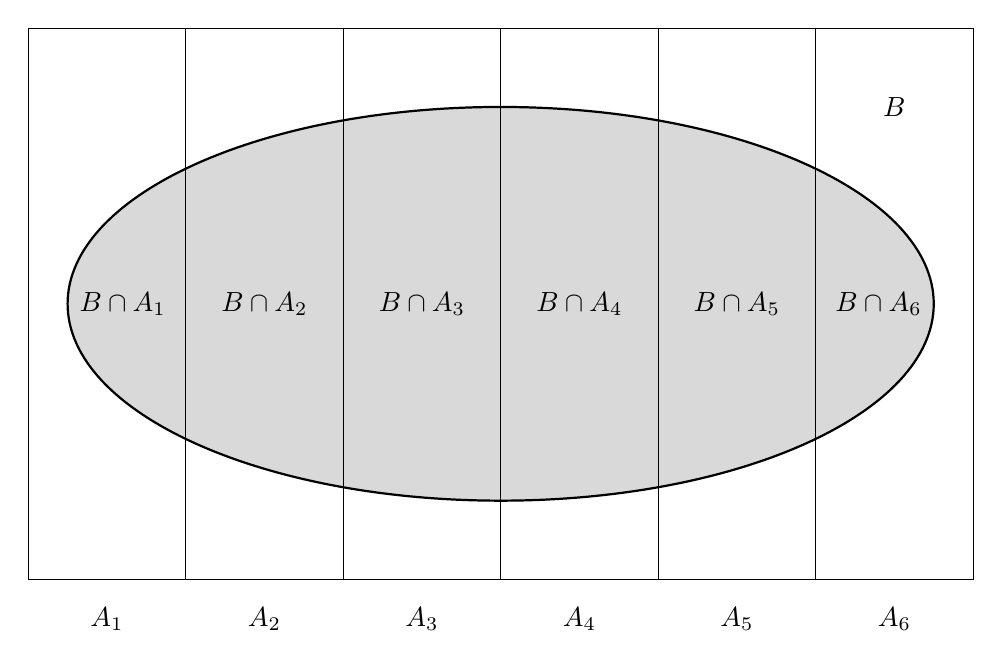
\begin{tikzpicture}
% 1. Dessiner le grand rectangle et les lignes verticales de partition
\draw (0,0) rectangle (12,7);

% 3. Dessiner une grande ellipse pour la forme B
\filldraw[
    fill=gray!30, % Remplissage gris clair
    thick % Trait épais pour le contour
] (6, 3.5) ellipse (5.5cm and 2.5cm); % Centre (6,3.5), rayon x=5.5cm, rayon y=2.5cm

\foreach \x in {2,4,6,8,10} {
    \draw (\x,0) -- (\x,7);
}

% 2. Placer les étiquettes A_1, A_2, ... en bas
\foreach \i [evaluate=\i as \xpos using \i*2-1] in {1,...,6} {
    \node at (\xpos, -0.5) {$A_{\i}$};
}

% 4. Placer l'étiquette pour l'ensemble B
\node at (11, 6) {$B$}; % Ajusté pour être au-dessus de l'ellipse

% 5. Placer les étiquettes pour les intersections B ∩ A_i, toutes au même niveau
\node at (1.2, 3.5) {$B \cap A_1$};
\node at (3, 3.5) {$B \cap A_2$};
\node at (5, 3.5) {$B \cap A_3$};
\node at (7, 3.5) {$B \cap A_4$};
\node at (9, 3.5) {$B \cap A_5$};
\node at (10.8, 3.5) {$B \cap A_6$};
\end{tikzpicture}
\end{center}
\end{intuitionbox}

L'exemple de l'usine est un cas d'école pour cette formule :

\begin{examplebox}
Une usine possède trois machines, M1, M2, et M3, qui produisent respectivement 50\%, 30\% et 20\% des articles. Leurs taux de production défectueuse sont de 4\%, 2\% et 5\%. Quelle est la probabilité qu'un article choisi au hasard soit défectueux ?
Soit $D$ l'événement "l'article est défectueux". Les machines forment une partition avec $P(M1)=0.5$, $P(M2)=0.3$, et $P(M3)=0.2$. Les probabilités conditionnelles de défaut sont $P(D|M1)=0.04$, $P(D|M2)=0.02$, et $P(D|M3)=0.05$.
En appliquant la formule, on obtient :
$P(D) = P(D|M1)P(M1) + P(D|M2)P(M2) + P(D|M3)P(M3) = (0.04 \times 0.5) + (0.02 \times 0.3) + (0.05 \times 0.2) = 0.02 + 0.006 + 0.01 = 0.036$.
La probabilité qu'un article soit défectueux est de 3.6\%.
\end{examplebox}

Maintenant, nous pouvons combiner la Règle de Bayes et la Formule des Probabilités Totales pour résoudre des problèmes complexes, comme celui du dépistage médical.

\begin{examplebox}[Application Combinée : Bayes et Probabilités Totales]
Une maladie touche 1\% de la population ($P(M) = 0.01$). Un test de dépistage est fiable à 95\% : il est positif pour 95\% des malades ($P(T|M)=0.95$) et négatif pour 95\% des non-malades, ce qui implique un taux de faux positifs de $P(T|\neg M) = 0.05$.
Une personne est testée positive. Quelle est la probabilité qu'elle soit réellement malade, $P(M|T)$ ?

On cherche $P(M|T) = \frac{P(T|M)P(M)}{P(T)}$.

D'abord, on calcule $P(T)$ avec la formule des probabilités totales (la partition est $\{M, \neg M\}$) :
$P(T) = P(T|M)P(M) + P(T|\neg M)P(\neg M) = (0.95 \times 0.01) + (0.05 \times 0.99) = 0.0095 + 0.0495 = 0.059$.

Ensuite, on applique la règle de Bayes : $P(M|T) = \frac{0.95 \times 0.01}{0.059} \approx 0.161$.
Malgré un test positif, il n'y a que 16.1\% de chance que la personne soit malade.
\end{examplebox}

\subsection{Règle de Bayes avec Conditionnement Additionnel}

Les règles que nous venons de voir (Bayes, Probabilités Totales) fonctionnent aussi si nous avons déjà une information de base $E$.

\begin{theorembox}[Règle de Bayes avec conditionnement additionnel]
À condition que $P(A \cap E) > 0$ et $P(B \cap E) > 0$, nous avons :
$$P(A|B, E) = \frac{P(B|A, E)P(A|E)}{P(B|E)}$$
\end{theorembox}

La preuve consiste à appliquer la définition de la probabilité conditionnelle à un univers déjà restreint par $E$.

\begin{proofbox}
La preuve est identique à celle de la règle de Bayes standard, mais en appliquant la définition de la probabilité conditionnelle à un univers restreint $E$.
$$P(A|B, E) = P(A|(B \cap E)) = \frac{P(A \cap (B \cap E))}{P(B \cap E)}$$
$$P(B|A, E) = P(B|(A \cap E)) = \frac{P(B \cap (A \cap E))}{P(A \cap E)}$$
De la première équation : $P(A \cap B \cap E) = P(A|B, E)P(B \cap E)$.
De la seconde : $P(A \cap B \cap E) = P(B|A, E)P(A \cap E)$.
En égalisant : $P(A|B, E)P(B \cap E) = P(B|A, E)P(A \cap E)$.
D'où : $P(A|B, E) = \frac{P(B|A, E)P(A \cap E)}{P(B \cap E)}$.
En utilisant $P(X \cap Y) = P(X|Y)P(Y)$, on a $P(A \cap E) = P(A|E)P(E)$ et $P(B \cap E) = P(B|E)P(E)$.
$$P(A|B, E) = \frac{P(B|A, E)P(A|E)P(E)}{P(B|E)P(E)} = \frac{P(B|A, E)P(A|E)}{P(B|E)}$$
\end{proofbox}

Cette formule peut sembler intimidante, mais elle signifie simplement que nous appliquons la même logique dans un "sous-monde" :

\begin{intuitionbox}
Cette formule est simplement la règle de Bayes standard, mais appliquée à l'intérieur d'un univers que l'on a déjà "rétréci".

Imaginez que vous recevez une information \textbf{E} qui élimine une grande partie des possibilités. C'est votre nouveau point de départ, votre monde est plus petit. Toutes les probabilités que vous calculez désormais sont relatives à ce monde restreint.

Dans ce nouveau monde, vous recevez une autre information, l'évidence \textbf{B}. La règle de Bayes conditionnelle vous permet alors de mettre à jour votre croyance sur un événement \textbf{A}, en utilisant exactement la même logique que la règle de Bayes classique, mais en vous assurant que chaque calcul reste confiné à l'intérieur des frontières de l'univers défini par \textbf{E}.
\end{intuitionbox}

\subsection{Formule des Probabilités Totales avec Conditionnement Additionnel}

De même, la loi des probabilités totales s'adapte à ce nouvel univers restreint.

\begin{theorembox}[Formule des probabilités totales avec conditionnement additionnel]
Soit $A_1, \dots, A_n$ une partition de $S$. À condition que $P(A_i \cap E) > 0$ pour tout $i$, nous avons :
$$P(B|E) = \sum_{i=1}^{n} P(B|A_i, E)P(A_i|E)$$
\end{theorembox}

La démonstration est une application directe de la formule standard, mais à l'intérieur de l'univers $E$.

\begin{proofbox}
La preuve suit celle de la formule des probabilités totales standard, mais tout est conditionné par $E$.
Soit $P_E(\cdot)$ une mesure de probabilité définie par $P_E(X) = P(X|E)$.
Les $A_i$ forment une partition de $S$, donc les $(A_i \cap E)$ forment une partition de $E$.
On applique la formule standard à $B \cap E$ :
$$P(B|E) = \sum_{i=1}^{n} P(B \cap A_i | E)$$
Par la définition de la probabilité conditionnelle :
$$P(B \cap A_i | E) = \frac{P(B \cap A_i \cap E)}{P(E)}$$
Et $P(B|A_i, E)P(A_i|E) = \frac{P(B \cap A_i \cap E)}{P(A_i \cap E)} \times \frac{P(A_i \cap E)}{P(E)} = \frac{P(B \cap A_i \cap E)}{P(E)}$
Les deux termes sont égaux, donc :
$$P(B|E) = \sum_{i=1}^{n} P(B|A_i, E)P(A_i|E)$$
\end{proofbox}

L'exemple visuel de la carte au trésor illustre parfaitement cette double-conditionnalité :

\begin{intuitionbox}
\begin{center}
\begin{tikzpicture}
  % Matrice principale, nommée "m"
  \matrix (m) [
    matrix of nodes,
    row sep = -\pgflinewidth,
    column sep = -\pgflinewidth,
    nodes={
      rectangle, draw=black, anchor=center,
      text height=4ex, text depth=0.5ex, minimum width=4em, fill=intuitionColor!10
    }
  ]
  {
    | |              & | |              & |[red_hatch]|    & | |              & | |              & | |            \\
    |[red_hatch]|    & |[purple_hatch]| & |[purple_hatch]| & | |              & |[red_hatch]|    & |[red_hatch]|  \\
    |[red_hatch]|    & |[blue_hatch]|   & |[red_hatch]|    & |[red_hatch]|    & |[red_hatch]|    & | |            \\
  };

  %  DÉLIMITATION DES COLONNES AVEC ACCOLADES 
  \draw [decorate, decoration={brace, amplitude=5pt, raise=4mm}]
    (m-1-1.north west) -- (m-1-2.north east) 
    node [midway, yshift=8mm, font=\bfseries] {A1};
    
  \draw [decorate, decoration={brace, amplitude=5pt, raise=4mm}]
    (m-1-3.north west) -- (m-1-4.north east) 
    node [midway, yshift=8mm, font=\bfseries] {A2};
    
  \draw [decorate, decoration={brace, amplitude=5pt, raise=4mm}]
    (m-1-5.north west) -- (m-1-6.north east) 
    node [midway, yshift=8mm, font=\bfseries] {A3};
\end{tikzpicture}
\end{center}
Imaginez que le graphique ci-dessus représente la carte d'un trésor. La carte est partitionnée en trois grandes régions : \textbf{A1}, \textbf{A2}, et \textbf{A3}. Sur cette carte, on a identifié deux types de terrains : une \textbf{zone marécageuse} (événement E, hachures rouges) qui s'étend sur \textbf{10 parcelles}, et une \textbf{zone près d'un vieux chêne} (événement B, hachures bleues) qui couvre \textbf{3 parcelles}.

On vous donne un premier indice : "Le trésor est dans la zone marécageuse (E)". Votre univers de recherche se réduit instantanément à ces 10 parcelles rouges. Puis, on vous donne un second indice : "Le trésor est aussi près d'un chêne (B)". Votre recherche se concentre alors sur les parcelles qui sont à la fois marécageuses et proches d'un chêne (les cases violettes, $B \cap E$).

La question est : "Sachant que le trésor est dans une parcelle violette, quelle est la probabilité qu'il se trouve dans la région A2 ?". On cherche donc $P(A_2 | B, E)$. La règle de Bayes nous permet de le calculer.

\textbf{Calcul des termes nécessaires :} D'abord, nous devons évaluer les probabilités à l'intérieur du "monde marécageux" (sachant E).

La \textbf{vraisemblance} est $P(B|A_2, E)$. En se limitant aux 4 parcelles marécageuses de la région A2, une seule est aussi près d'un chêne. Donc, $P(B|A_2, E) = 1/4$.

La \textbf{probabilité a priori} est $P(A_2|E)$. Sur les 10 parcelles marécageuses, 4 sont dans la région A2. Donc, $P(A_2|E) = 4/10$.

L'\textbf{évidence}, $P(B|E)$, est la probabilité de trouver un chêne dans l'ensemble de la zone marécageuse. On peut la calculer avec la formule des probabilités totales :
$$P(B|E) = P(B|A_1, E)P(A_1|E) + P(B|A_2, E)P(A_2|E) + P(B|A_3, E)P(A_3|E)$$
$$P(B|E) = (\frac{1}{3} \times \frac{3}{10}) + (\frac{1}{4} \times \frac{4}{10}) + (0 \times \frac{3}{10}) = \frac{1}{10} + \frac{1}{10} = \frac{2}{10}$$

\textbf{Application de la règle de Bayes :} Maintenant, nous assemblons le tout.
$$P(A_2|B, E) = \frac{P(B|A_2, E)P(A_2|E)}{P(B|E)} = \frac{(1/4) \times (4/10)}{2/10} = \frac{1/10}{2/10} = \frac{1}{2}$$
L'intuition confirme le calcul : sachant que le trésor est sur une parcelle violette, et qu'il n'y en a que deux (une en A1, une en A2), il y a bien une chance sur deux qu'il se trouve dans la région A2.
\end{intuitionbox}

\subsection{Indépendance de Deux Événements}

Le concept d'indépendance est un cas spécial de probabilité conditionnelle où l'information $B$ n'a aucun effet sur la probabilité de $A$.

\begin{definitionbox}[Indépendance de deux événements]
Les événements $A$ et $B$ sont indépendants si :
$$P(A \cap B) = P(A)P(B)$$
Si $P(A) > 0$ et $P(B) > 0$, cela est équivalent à :
$$P(A|B) = P(A)$$
\end{definitionbox}

En d'autres termes :

\begin{intuitionbox}
L'indépendance est l'absence d'information. Si deux événements sont indépendants, apprendre que l'un s'est produit ne change absolument rien à la probabilité de l'autre. Savoir qu'il pleut à Tokyo ($B$) ne modifie pas la probabilité que vous obteniez pile en lançant une pièce ($A$).
\end{intuitionbox}

\subsection{Indépendance Conditionnelle}

Attention : l'indépendance n'est pas la même chose que l'exclusion mutuelle. Il faut aussi se méfier de l'indépendance qui n'est qu'apparente, ou qui dépend d'une autre condition.

\begin{definitionbox}[Indépendance Conditionnelle]
Les événements $A$ et $B$ sont dits conditionnellement indépendants étant donné $E$ si :
$$P(A \cap B | E) = P(A|E)P(B|E)$$
\end{definitionbox}

C'est un concept subtil mais crucial :

\begin{intuitionbox}
L'indépendance peut apparaître ou disparaître quand on observe un autre événement. Par exemple, vos notes en maths ($A$) et en physique ($B$) ne sont probablement pas indépendantes. Mais si l'on sait que vous avez beaucoup travaillé ($E$), alors vos notes en maths et en physique pourraient devenir indépendantes. L'information "vous avez beaucoup travaillé" explique la corrélation ; une fois qu'on la connaît, connaître votre note en maths n'apporte plus d'information sur votre note en physique.
\end{intuitionbox}

\subsection{Le Problème de Monty Hall}

Pour tester notre compréhension de tous ces concepts, le problème de Monty Hall est un exercice incontournable. Il met en lumière à quel point notre intuition sur la mise à jour des probabilités peut être faussée.

\begin{remarquebox}[Le problème de Monty Hall]
Imaginez que vous êtes à un jeu télévisé. Face à vous se trouvent trois portes fermées. Derrière l'une d'elles se trouve une voiture, et derrière les deux autres, des chèvres.
\begin{enumerate}
    \item Vous choisissez une porte (disons, la porte n°1).
    \item L'animateur, qui sait où se trouve la voiture, ouvre une autre porte (par exemple, la n°3) derrière laquelle se trouve une chèvre.
    \item Il vous demande alors : "Voulez-vous conserver votre choix initial (porte n°1) ou changer pour l'autre porte restante (la n°2) ?"
\end{enumerate}
\textbf{Question :} Avez-vous intérêt à changer de porte ? Votre probabilité de gagner la voiture est-elle plus grande si vous changez, si vous ne changez pas, ou est-elle la même dans les deux cas ?
\end{remarquebox}

La réponse est contre-intuitive pour la plupart des gens, mais mathématiquement claire.

\begin{correctionbox}[Solution du problème de Monty Hall]
La réponse est sans équivoque : il faut \textbf{toujours changer de porte}. Cette stratégie fait passer la probabilité de gagner de $1/3$ à $2/3$. L'intuition et la preuve ci-dessous détaillent ce résultat surprenant.
\end{correctionbox}

Pourquoi ? L'erreur est de penser que l'animateur agit au hasard.

\begin{intuitionbox}[Le secret : l'information de l'animateur]
L'erreur commune est de supposer qu'il reste deux portes avec une chance égale de $1/2$. Cela ignore une information capitale : le choix de l'animateur n'est \textbf{pas aléatoire}. Il sait où se trouve la voiture et ouvrira toujours une porte perdante.

Le raisonnement correct se déroule en deux temps. D'abord, votre choix initial a $\mathbf{1/3}$ de chance d'être correct. Cela implique qu'il y a $\mathbf{2/3}$ de chance que la voiture soit derrière l'une des \textit{deux autres portes}. Ensuite, lorsque l'animateur ouvre l'une de ces deux portes, il ne fait que vous montrer où la voiture n'est \textit{pas} dans cet ensemble. La probabilité de $2/3$ se \textbf{concentre} alors entièrement sur la seule porte qu'il a laissée fermée. Changer de porte revient à miser sur cette probabilité de $2/3$.
\end{intuitionbox}

La preuve la plus claire est de suivre les stratégies :

\begin{proofbox}[Preuve par l'arbre de décision]
L'analyse de la meilleure stratégie peut être visualisée à l'aide de l'arbre de décision ci-dessous. Il décompose le problème en deux scénarios initiaux : avoir choisi la bonne porte (probabilité $1/3$) ou une mauvaise porte (probabilité $2/3$).

\vspace{0.5cm}
\begin{center}
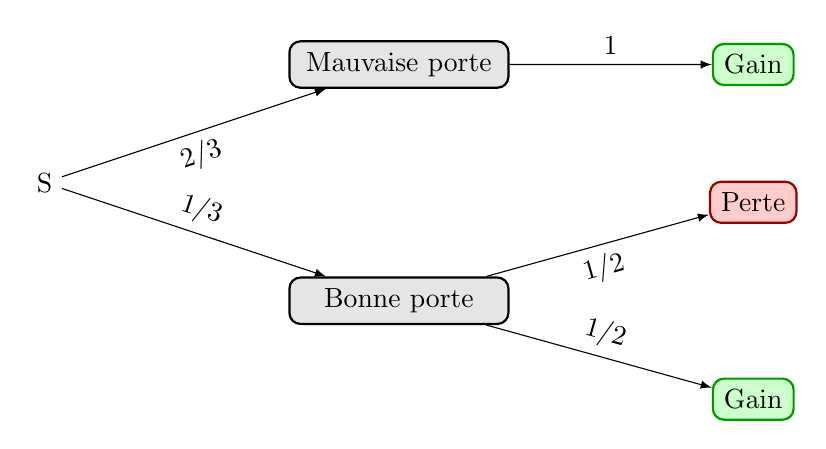
\begin{tikzpicture}[
  grow=right,
  level distance=4.5cm,
  level 1/.style={sibling distance=3cm},
  level 2/.style={sibling distance=2.5cm},
  edge from parent/.style={draw, -latex},
  %  Définition des styles pour les cadres 
  porte_style/.style={rectangle, rounded corners, draw=black, fill=gray!20, thick, inner sep=4pt, text width=2.5cm, align=center},
  gain_style/.style={rectangle, rounded corners, draw=green!60!black, fill=green!20, thick, inner sep=4pt},
  perte_style/.style={rectangle, rounded corners, draw=red!60!black, fill=red!20, thick, inner sep=4pt}
]

\node {S}
    %  Branche du haut 
    child {
        node[porte_style] {Bonne porte}
        child {
            node[gain_style] {Gain}
            edge from parent
            node[above, sloped] {$1/2$}
        }
        child {
            node[perte_style] {Perte}
            edge from parent
            node[below, sloped] {$1/2$}
        }
        edge from parent
        node[above, sloped] {1/3}
    }
    %  Branche du bas 
    child {
        node[porte_style] {Mauvaise porte}
        child {
            node[gain_style] {Gain}
            edge from parent
            node[above, sloped] {1}
        }
        edge from parent
        node[below, sloped] {2/3}
    };
\end{tikzpicture}
\end{center}
\vspace{0.5cm}

\noindent\textbf{Analyse de l'arbre :}

\noindent\textbf{Branche du bas (cas le plus probable) :}
Avec une probabilité de $\mathbf{2/3}$, votre choix initial se porte sur une "Mauvaise porte". L'animateur est alors obligé de révéler l'autre porte perdante. La seule porte restante est donc la bonne. L'arbre montre que cela mène à un "Gain" avec une probabilité de $\mathbf{1}$. Ce chemin correspond au résultat de la stratégie \textbf{"Changer"}.

\noindent\textbf{Branche du haut (cas le moins probable) :}
Avec une probabilité de $\mathbf{1/3}$, vous avez choisi la "Bonne porte" du premier coup. L'arbre se divise alors en deux issues équiprobables ($1/2$ chacune). L'issue "Gain" correspond à la stratégie \textbf{"Garder"} votre choix initial, tandis que l'issue "Perte" correspond à la stratégie \textbf{"Changer"} pour la porte perdante restante.

\noindent\textbf{Conclusion :}
Pour évaluer la meilleure stratégie, il suffit de sommer les probabilités de gain. La \textbf{probabilité de gain en changeant} est de $\mathbf{2/3}$, car vous gagnez uniquement si votre choix initial était mauvais (branche du bas). La \textbf{probabilité de gain en gardant} est de $\mathbf{1/3}$, car vous gagnez uniquement si votre choix initial était bon (branche "Gain" du haut). La stratégie optimale est donc bien de toujours changer de porte.
\end{proofbox}

\subsection{Exercices}

%  Concepts de Base et Règle du Produit 

\begin{exercicebox}[Exercice 1 : Dés et Probabilité Conditionnelle Simple]
On lance deux dés équilibrés à 6 faces.
\begin{enumerate}
    \item Quelle est la probabilité que la somme des dés soit 8 ?
    \item Sachant que le premier dé a donné un 3, quelle est la probabilité que la somme soit 8 ?
    \item Sachant que la somme est 8, quelle est la probabilité que le premier dé ait donné un 3 ?
\end{enumerate}
\end{exercicebox}

\begin{exercicebox}[Exercice 2 : Tirage de Cartes (Sans Remise)]
On tire deux cartes successivement et sans remise d'un jeu standard de 52 cartes.
\begin{enumerate}
    \item Quelle est la probabilité que la deuxième carte soit un Roi, sachant que la première était un Roi ?
    \item Quelle est la probabilité de tirer deux Rois ?
\end{enumerate}
\end{exercicebox}

\begin{exercicebox}[Exercice 3 : Urne (Règle du Produit)]
Une urne contient 7 boules rouges et 3 boules bleues. On tire deux boules successivement et sans remise.
\begin{enumerate}
    \item Quelle est la probabilité que la première boule soit rouge ?
    \item Quelle est la probabilité que la deuxième boule soit bleue, sachant que la première était rouge ?
    \item Quelle est la probabilité de tirer une boule rouge puis une boule bleue ?
\end{enumerate}
\end{exercicebox}

\begin{exercicebox}[Exercice 4 : Famille (Condition Simple)]
Une famille a deux enfants. On suppose que la probabilité d'avoir un garçon (G) ou une fille (F) est la même (0.5) et que les naissances sont indépendantes.
\begin{enumerate}
    \item Quel est l'univers $S$ des possibilités ?
    \item Sachant que l'aîné est un garçon, quelle est la probabilité que la famille ait deux garçons ?
\end{enumerate}
\end{exercicebox}

\begin{exercicebox}[Exercice 5 : Famille (Condition "Au Moins")]
En utilisant le même scénario que l'exercice 4 (famille de deux enfants) :
Sachant qu'il y a \textit{au moins un} garçon dans la famille, quelle est la probabilité que la famille ait deux garçons ?
\end{exercicebox}

%  Indépendance 

\begin{exercicebox}[Exercice 6 : Indépendance (Dés)]
On lance deux dés équilibrés.
Soit $A$ l'événement "le premier dé donne 3" et $B$ l'événement "la somme des deux dés est 7".
Les événements $A$ et $B$ sont-ils indépendants ? Justifiez par le calcul.
\end{exercicebox}

\begin{exercicebox}[Exercice 7 : Indépendance (Cartes)]
On tire une carte d'un jeu de 52 cartes.
Soit $A$ l'événement "la carte est un Roi" et $B$ l'événement "la carte est un Cœur".
Les événements $A$ et $B$ sont-ils indépendants ?
\end{exercicebox}

\begin{exercicebox}[Exercice 8 : Indépendance vs Exclusion Mutuelle]
Soient $A$ et $B$ deux événements avec $P(A)=0.5$ et $P(B)=0.3$.
\begin{enumerate}
    \item Si $A$ et $B$ sont mutuellement exclusifs (disjoints), sont-ils indépendants ?
    \item Si $A$ et $B$ sont indépendants, quelle est $P(A \cup B)$ ?
\end{enumerate}
\end{exercicebox}

%  Formule des Probabilités Totales (LTP) 

\begin{exercicebox}[Exercice 9 : LTP (Deux Urnes)]
L'urne U1 contient 2 boules noires et 3 boules blanches. L'urne U2 contient 4 boules noires et 1 boule blanche.
On choisit une urne au hasard (chaque urne a 50\% de chance d'être choisie), puis on tire une boule de cette urne.
Quelle est la probabilité de tirer une boule blanche ?
\end{exercicebox}

\begin{exercicebox}[Exercice 10 : LTP (Usine)]
Une usine utilise deux machines, M1 et M2, pour produire des pièces. M1 produit 40\% des pièces et M2 produit 60\%. 5\% des pièces de M1 sont défectueuses, et 2\% des pièces de M2 sont défectueuses.
Si l'on choisit une pièce au hasard dans la production totale, quelle est la probabilité qu'elle soit défectueuse ?
\end{exercicebox}

\begin{exercicebox}[Exercice 11 : LTP (Pièce de Monnaie Inconnue)]
On a deux pièces. La pièce A est équilibrée ($P(\text{Pile})=0.5$). La pièce B est truquée ($P(\text{Pile})=0.8$).
On choisit une pièce au hasard et on la lance. Quelle est la probabilité d'obtenir Pile ?
\end{exercicebox}

%  Règle de Bayes 

\begin{exercicebox}[Exercice 12 : Bayes (Test Médical)]
Une maladie touche 1 personne sur 1000 ($P(M)=0.001$). Un test de dépistage donne un résultat positif chez 98\% des personnes malades ($P(T|M)=0.98$). Il donne aussi un résultat positif (un "faux positif") chez 3\% des personnes non malades ($P(T|\neg M)=0.03$).
Une personne reçoit un test positif. Quelle est la probabilité qu'elle soit réellement malade ?
\end{exercicebox}

\begin{exercicebox}[Exercice 13 : Bayes (Inversion d'Urnes)]
Reprenons le scénario de l'exercice 9 (U1 avec 2N/3B, U2 avec 4N/1B).
On a tiré une boule et on constate qu'elle est blanche. Quelle est la probabilité qu'elle provienne de l'urne U1 ?
\end{exercicebox}

\begin{exercicebox}[Exercice 14 : Bayes (Spam)]
Dans une boîte de réception, 60\% des emails sont des spams. 70\% des spams contiennent le mot "gratuit". Seuls 10\% des emails légitimes contiennent le mot "gratuit".
Vous recevez un email qui contient le mot "gratuit". Quelle est la probabilité que ce soit un spam ?
\end{exercicebox}

\begin{exercicebox}[Exercice 15 : Bayes (Usine Inversée)]
Reprenons le scénario de l'exercice 10 (M1: 40\% prod, 5\% défaut; M2: 60% prod, 2% défaut).
On trouve une pièce défectueuse. Quelle est la probabilité qu'elle ait été produite par la machine M1 ?
\end{exercicebox}

%  Règle de la Chaîne et Problèmes Combinés 

\begin{exercicebox}[Exercice 16 : Règle de la Chaîne (3 Cartes)]
On tire 3 cartes successivement et sans remise d'un jeu de 52 cartes.
Quelle est la probabilité de tirer 3 Piques ?
\end{exercicebox}

\begin{exercicebox}[Exercice 17 : Problème de Monty Hall (Calcul)]
En utilisant la formalisation du problème de Monty Hall (vous choisissez la Porte 1, la voiture est en $V \in \{1, 2, 3\}$, l'animateur ouvre $H \in \{2, 3\}$) :
Calculez $P(V=1 | H=3)$ (la probabilité que la voiture soit derrière votre porte, sachant que l'animateur a ouvert la 3). Supposez que $P(V=i)=1/3$ pour $i=1,2,3$.
\end{exercicebox}

\begin{exercicebox}[Exercice 18 : Bayes avec Mise à Jour (Pièce Truquée)]
Reprenons l'exercice 11 (Pièce A équilibrée, Pièce B truquée $P(\text{Pile})=0.8$).
On choisit une pièce au hasard. On la lance deux fois et on obtient Pile, puis Pile (PP).
Quelle est la probabilité que l'on ait choisi la pièce truquée (Pièce B) ?
\end{exercicebox}

\begin{exercicebox}[Exercice 19 : Indépendance Conditionnelle (Dés)]
On lance deux dés, $D_1$ et $D_2$. Soit $S = D_1 + D_2$ leur somme.
Soit $A$ l'événement "$D_1 = 1$", $B$ l'événement "$D_2 = 1$".
$A$ et $B$ sont indépendants. Sont-ils indépendants conditionnellement à l'événement $C = \{S = 2\}$ ?
\end{exercicebox}

\begin{exercicebox}[Exercice 20 : Jeu Séquentiel]
Alice et Bob jouent à un jeu. Ils lancent un dé à tour de rôle, en commençant par Alice. Le premier qui obtient un 6 gagne.
Quelle est la probabilité qu'Alice gagne ?
\end{exercicebox}

\subsection{Corrections des Exercices}

%  Corrections : Concepts de Base et Règle du Produit 

\begin{correctionbox}[Correction Exercice 1 : Dés et Probabilité Conditionnelle Simple]
L'univers $S$ a $|S| = 6 \times 6 = 36$ issues.

1.  Soit $A$ l'événement "la somme est 8". $A = \{(2,6), (3,5), (4,4), (5,3), (6,2)\}$.
    $|A|=5$, donc $P(A) = 5/36$.

2.  Soit $B$ l'événement "le premier dé donne 3". $B = \{(3,1), (3,2), (3,3), (3,4), (3,5), (3,6)\}$.
    On cherche $P(A|B)$. Sachant $B$, l'univers est réduit à ces 6 issues. Parmi celles-ci, seule l'issue $(3,5)$ donne une somme de 8.
    Donc, $P(A|B) = 1/6$.
    *Par formule :* $A \cap B = \{(3,5)\}$, $P(A \cap B) = 1/36$. $P(B) = 6/36 = 1/6$.
    $P(A|B) = \frac{P(A \cap B)}{P(B)} = \frac{1/36}{6/36} = 1/6$.

3.  On cherche $P(B|A)$. Sachant $A$, l'univers est réduit aux 5 issues de $A$. Parmi celles-ci, seule l'issue $(3,5)$ a 3 sur le premier dé.
    Donc, $P(B|A) = 1/5$.
    *Par formule :* $P(B|A) = \frac{P(A \cap B)}{P(A)} = \frac{1/36}{5/36} = 1/5$.
\end{correctionbox}

\begin{correctionbox}[Correction Exercice 2 : Tirage de Cartes (Sans Remise)]
Soit $K_1$ l'événement "Roi au 1er tirage" et $K_2$ "Roi au 2e tirage".

1.  On cherche $P(K_2|K_1)$. Si $K_1$ s'est produit, il reste 51 cartes dans le jeu, dont $4-1=3$ Rois.
    $P(K_2|K_1) = 3/51 = 1/17$.

2.  On cherche $P(K_1 \cap K_2)$. On utilise la règle du produit :
    $P(K_1 \cap K_2) = P(K_1) \times P(K_2|K_1)$
    $P(K_1) = 4/52 = 1/13$.
    $P(K_1 \cap K_2) = (4/52) \times (3/51) = (1/13) \times (1/17) = 1/221$.
\end{correctionbox}

\begin{correctionbox}[Correction Exercice 3 : Urne (Règle du Produit)]
Urne avec 7 Rouges (R) et 3 Bleues (B). Total = 10.
Soit $R_1$ "Rouge au 1er tirage" et $B_2$ "Bleue au 2e tirage".

1.  $P(R_1) = 7/10$.
2.  On cherche $P(B_2|R_1)$. Si $R_1$ s'est produit, il reste 9 boules (6R, 3B).
    $P(B_2|R_1) = 3/9 = 1/3$.
3.  On cherche $P(R_1 \cap B_2)$.
    $P(R_1 \cap B_2) = P(R_1) \times P(B_2|R_1) = (7/10) \times (1/3) = 7/30$.
\end{correctionbox}

\begin{correctionbox}[Correction Exercice 4 : Famille (Condition Simple)]
1.  L'univers est $S = \{GG, GF, FG, FF\}$, où le premier enfant est l'aîné. $|S|=4$, chaque issue a une probabilité de 1/4.
2.  Soit $A$ l'événement "l'aîné est un garçon" : $A = \{GG, GF\}$. $P(A) = 2/4 = 1/2$.
    Soit $B$ l'événement "la famille a deux garçons" : $B = \{GG\}$. $P(B) = 1/4$.
    On cherche $P(B|A)$. L'événement $A \cap B = \{GG\}$. $P(A \cap B) = 1/4$.
    $P(B|A) = \frac{P(A \cap B)}{P(A)} = \frac{1/4}{1/2} = 1/2$.
\end{correctionbox}

\begin{correctionbox}[Correction Exercice 5 : Famille (Condition "Au Moins")]
Soit $B$ l'événement "la famille a deux garçons" : $B = \{GG\}$.
Soit $C$ l'événement "il y a au moins un garçon" : $C = \{GG, GF, FG\}$. $P(C) = 3/4$.
On cherche $P(B|C)$.
L'événement $B \cap C = \{GG\}$. $P(B \cap C) = 1/4$.
$P(B|C) = \frac{P(B \cap C)}{P(C)} = \frac{1/4}{3/4} = 1/3$.
*Intuition :* L'univers de $C$ est $\{GG, GF, FG\}$. Parmi ces 3 issues équiprobables, une seule est $GG$.
\end{correctionbox}

%  Corrections : Indépendance 

\begin{correctionbox}[Correction Exercice 6 : Indépendance (Dés)]
$A$ = "premier dé = 3". $P(A) = 6/36 = 1/6$.
$B$ = "somme = 7". $B = \{(1,6), (2,5), (3,4), (4,3), (5,2), (6,1)\}$. $P(B) = 6/36 = 1/6$.
$A \cap B$ = "premier dé = 3 ET somme = 7" = $\%(3,4)\}$. $P(A \cap B) = 1/36$.
On teste si $P(A \cap B) = P(A)P(B)$.
$P(A)P(B) = (1/6) \times (1/6) = 1/36$.
Puisque $P(A \cap B) = P(A)P(B)$, les événements $A$ et $B$ sont indépendants.
\end{correctionbox}

\begin{correctionbox}[Correction Exercice 7 : Indépendance (Cartes)]
$A$ = "Roi". $P(A) = 4/52 = 1/13$.
$B$ = "Cœur". $P(B) = 13/52 = 1/4$.
$A \cap B$ = "Roi de Cœur". $P(A \cap B) = 1/52$.
On teste si $P(A \cap B) = P(A)P(B)$.
$P(A)P(B) = (1/13) \times (1/4) = 1/52$.
Puisque $P(A \cap B) = P(A)P(B)$, les événements $A$ et $B$ sont indépendants.
\end{correctionbox}

\begin{correctionbox}[Correction Exercice 8 : Indépendance vs Exclusion Mutuelle]
$P(A)=0.5, P(B)=0.3$.

1.  Si $A$ et $B$ sont mutuellement exclusifs, $A \cap B = \emptyset$, donc $P(A \cap B) = 0$.
    Pour qu'ils soient indépendants, il faudrait $P(A \cap B) = P(A)P(B) = 0.5 \times 0.3 = 0.15$.
    Puisque $0 \neq 0.15$, ils ne sont pas indépendants. (Deux événements non impossibles ne peuvent pas être à la fois mutuellement exclusifs et indépendants).

2.  Si $A$ et $B$ sont indépendants, $P(A \cap B) = P(A)P(B) = 0.15$.
    $P(A \cup B) = P(A) + P(B) - P(A \cap B) = 0.5 + 0.3 - 0.15 = 0.65$.
\end{correctionbox}

%  Corrections : Formule des Probabilités Totales (LTP) 

\begin{correctionbox}[Correction Exercice 9 : LTP (Deux Urnes)]
Soit $U_1$ et $U_2$ les événements "choisir l'urne 1" et "choisir l'urne 2". $P(U_1)=0.5, P(U_2)=0.5$.
Soit $W$ l'événement "tirer une boule blanche".
On a $P(W|U_1) = 3 / (2+3) = 3/5 = 0.6$.
On a $P(W|U_2) = 1 / (4+1) = 1/5 = 0.2$.
Par la formule des probabilités totales :
$P(W) = P(W|U_1)P(U_1) + P(W|U_2)P(U_2)$
$P(W) = (0.6 \times 0.5) + (0.2 \times 0.5) = 0.3 + 0.1 = 0.4$.
\end{correctionbox}

\begin{correctionbox}[Correction Exercice 10 : LTP (Usine)]
Soit $M_1$ et $M_2$ les machines. $P(M_1)=0.4, P(M_2)=0.6$.
Soit $D$ l'événement "la pièce est défectueuse".
On a $P(D|M_1) = 0.05$ et $P(D|M_2) = 0.02$.
Par la formule des probabilités totales :
$P(D) = P(D|M_1)P(M_1) + P(D|M_2)P(M_2)$
$P(D) = (0.05 \times 0.4) + (0.02 \times 0.6) = 0.020 + 0.012 = 0.032$.
La probabilité est de 3.2\%.
\end{correctionbox}

\begin{correctionbox}[Correction Exercice 11 : LTP (Pièce de Monnaie Inconnue)]
Soit $A$ "choisir pièce A" et $B$ "choisir pièce B". $P(A)=0.5, P(B)=0.5$.
Soit $H$ l'événement "obtenir Pile".
On a $P(H|A) = 0.5$ et $P(H|B) = 0.8$.
Par la formule des probabilités totales :
$P(H) = P(H|A)P(A) + P(H|B)P(B)$
$P(H) = (0.5 \times 0.5) + (0.8 \times 0.5) = 0.25 + 0.40 = 0.65$.
\end{correctionbox}

%  Corrections : Règle de Bayes 

\begin{correctionbox}[Correction Exercice 12 : Bayes (Test Médical)]
Soit $M$ "Malade" et $T$ "Test Positif".
$P(M) = 0.001$, donc $P(\neg M) = 0.999$.
$P(T|M) = 0.98$.
$P(T|\neg M) = 0.03$.
On cherche $P(M|T)$. Par la règle de Bayes : $P(M|T) = \frac{P(T|M)P(M)}{P(T)}$.

1.  Calculer $P(T)$ (dénominateur) avec la LTP :
    $P(T) = P(T|M)P(M) + P(T|\neg M)P(\neg M)$
    $P(T) = (0.98 \times 0.001) + (0.03 \times 0.999) = 0.00098 + 0.02997 = 0.03095$.

2.  Appliquer la règle de Bayes :
    $P(M|T) = \frac{0.00098}{0.03095} \approx 0.03166$.
    Il n'y a que 3.17\% de chance que la personne soit malade, même avec un test positif.
\end{correctionbox}

\begin{correctionbox}[Correction Exercice 13 : Bayes (Inversion d'Urnes)]
D'après l'exercice 9, on a :
$P(W) = 0.4$ (prob. totale de tirer une blanche).
$P(W|U_1) = 0.6$.
$P(U_1) = 0.5$.
On cherche $P(U_1|W)$. Par la règle de Bayes :
$P(U_1|W) = \frac{P(W|U_1)P(U_1)}{P(W)} = \frac{0.6 \times 0.5}{0.4} = \frac{0.3}{0.4} = 0.75$.
Sachant que la boule est blanche, il y a 75\% de chance qu'elle vienne de l'urne U1.
\end{correctionbox}

\begin{correctionbox}[Correction Exercice 14 : Bayes (Spam)]
Soit $S$ "Spam" et $G$ "Contient 'gratuit'".
$P(S) = 0.6$, donc $P(\neg S) = 0.4$.
$P(G|S) = 0.7$.
$P(G|\neg S) = 0.1$.
On cherche $P(S|G)$. Par la règle de Bayes : $P(S|G) = \frac{P(G|S)P(S)}{P(G)}$.

1.  Calculer $P(G)$ (dénominateur) avec la LTP :
    $P(G) = P(G|S)P(S) + P(G|\neg S)P(\neg S)$
    $P(G) = (0.7 \times 0.6) + (0.1 \times 0.4) = 0.42 + 0.04 = 0.46$.

2.  Appliquer la règle de Bayes :
    $P(S|G) = \frac{0.42}{0.46} \approx 0.913$.
    Il y a 91.3\% de chance que l'email soit un spam.
\end{correctionbox}

\begin{correctionbox}[Correction Exercice 15 : Bayes (Usine Inversée)]
D'après l'exercice 10, on a :
$P(D) = 0.032$ (prob. totale d'être défectueux).
$P(D|M_1) = 0.05$.
$P(M_1) = 0.4$.
On cherche $P(M_1|D)$. Par la règle de Bayes :
$P(M_1|D) = \frac{P(D|M_1)P(M_1)}{P(D)} = \frac{0.05 \times 0.4}{0.032} = \frac{0.02}{0.032} = 0.625$.
Sachant que la pièce est défectueuse, il y a 62.5\% de chance qu'elle vienne de M1.
\end{correctionbox}

%  Corrections : Règle de la Chaîne et Problèmes Combinés 

\begin{correctionbox}[Correction Exercice 16 : Règle de la Chaîne (3 Cartes)]
Soit $P_i$ l'événement "tirer un Pique au $i$-ème tirage". Il y a 13 Piques sur 52 cartes.
On cherche $P(P_1 \cap P_2 \cap P_3)$. On utilise la règle de la chaîne :
$P(P_1 \cap P_2 \cap P_3) = P(P_1) \times P(P_2|P_1) \times P(P_3|P_1 \cap P_2)$
$P(P_1) = 13/52$.
$P(P_2|P_1) = 12/51$ (il reste 12 Piques sur 51 cartes).
$P(P_3|P_1 \cap P_2) = 11/50$ (il reste 11 Piques sur 50 cartes).
$P = (13/52) \times (12/51) \times (11/50) = \frac{1}{4} \times \frac{4}{17} \times \frac{11}{50} = \frac{11}{17 \times 50} = 11/850 \approx 0.0129$.
\end{correctionbox}

\begin{correctionbox}[Correction Exercice 17 : Problème de Monty Hall (Calcul)]
On cherche $P(V=1 | H=3)$. On utilise la règle de Bayes :
$P(V=1 | H=3) = \frac{P(H=3 | V=1) P(V=1)}{P(H=3)}$.

*Numérateur :* $P(V=1) = 1/3$. $P(H=3 | V=1)$ est la probabilité que l'animateur ouvre la 3, sachant que vous avez choisi la 1 et que la voiture est en 1. Il peut ouvrir la 2 ou la 3 (deux chèvres). On suppose qu'il choisit au hasard : $P(H=3 | V=1) = 1/2$.
Numérateur = $(1/2) \times (1/3) = 1/6$.

*Dénominateur $P(H=3)$ par LTP (partition sur V) :*
$P(H=3) = P(H=3|V=1)P(V=1) + P(H=3|V=2)P(V=2) + P(H=3|V=3)P(V=3)$
- $P(H=3|V=1) = 1/2$ (calculé ci-dessus).
- $P(H=3|V=2) = 1$ (l'animateur doit ouvrir la 3, car vous avez choisi 1 et la voiture est en 2).
- $P(H=3|V=3) = 0$ (l'animateur ne peut pas ouvrir la porte 3 car elle contient la voiture).
$P(H=3) = (1/2 \times 1/3) + (1 \times 1/3) + (0 \times 1/3) = 1/6 + 1/3 + 0 = 1/2$.

*Résultat :* $P(V=1 | H=3) = \frac{1/6}{1/2} = 1/3$.
(La probabilité que la voiture soit derrière votre porte reste 1/3. La probabilité qu'elle soit derrière l'autre porte fermée (la 2) est $P(V=2|H=3) = 1 - P(V=1|H=3) = 2/3$. Il faut donc changer.)
\end{correctionbox}

\begin{correctionbox}[Correction Exercice 18 : Bayes avec Mise à Jour (Pièce Truquée)]
Soit $A$ "pièce A (équil.)" et $B$ "pièce B (truquée, p=0.8)". $P(A)=P(B)=0.5$.
Soit $E$ l'événement "obtenir Pile, Pile" (PP).
On cherche $P(B|E) = \frac{P(E|B)P(B)}{P(E)}$.

1.  Probabilités conditionnelles de l'évidence $E$ :
    $P(E|A) = P(\text{PP} | A) = 0.5 \times 0.5 = 0.25$ (indépendance des lancers).
    $P(E|B) = P(\text{PP} | B) = 0.8 \times 0.8 = 0.64$.

2.  Calculer $P(E)$ (dénominateur) avec la LTP :
    $P(E) = P(E|A)P(A) + P(E|B)P(B)$
    $P(E) = (0.25 \times 0.5) + (0.64 \times 0.5) = 0.125 + 0.320 = 0.445$.

3.  Appliquer la règle de Bayes :
    $P(B|E) = \frac{P(E|B)P(B)}{P(E)} = \frac{0.64 \times 0.5}{0.445} = \frac{0.32}{0.445} \approx 0.719$.
    Après avoir observé PP, la probabilité que ce soit la pièce truquée passe de 50\% à 71.9\%.
\end{correctionbox}

\begin{correctionbox}[Correction Exercice 19 : Indépendance Conditionnelle (Dés)]
$A = \{D_1=1\}$, $B = \{D_2=1\}$, $C = \{S=2\}$.
On teste si $P(A \cap B | C) = P(A|C) P(B|C)$.

L'événement $C = \{S=2\}$ ne peut se produire que d'une seule façon : $C = \{(1,1)\}$.
Donc, $C$ est l'événement $A \cap B$. $C \subseteq A$ et $C \subseteq B$.

Calculons les termes :
- $P(A|C) = P(A \cap C) / P(C)$. Puisque $C \subseteq A$, $A \cap C = C$.
  $P(A|C) = P(C) / P(C) = 1$.
- $P(B|C) = P(B \cap C) / P(C)$. Puisque $C \subseteq B$, $B \cap C = C$.
  $P(B|C) = P(C) / P(C) = 1$.
- $P(A \cap B | C) = P((A \cap B) \cap C) / P(C)$. Puisque $A \cap B = C$, $(A \cap B) \cap C = C$.
  $P(A \cap B | C) = P(C) / P(C) = 1$.

Test d'indépendance :
$P(A \cap B | C) = 1$.
$P(A|C) P(B|C) = 1 \times 1 = 1$.
Puisque $1=1$, les événements $A$ et $B$ sont bien indépendants conditionnellement à $C$.
*Intuition :* Sachant que la somme est 2, nous savons avec certitude que $D_1=1$ et $D_2=1$. Il n'y a plus d'aléa.
\end{correctionbox}

\begin{correctionbox}[Correction Exercice 20 : Jeu Séquentiel]
Soit $p=1/6$ la probabilité de gagner (obtenir un 6) et $q=5/6$ la probabilité de rater.
Alice gagne si elle réussit au tour 1, OU si (elle rate ET Bob rate) et elle réussit au tour 3, OU si (A rate, B rate, A rate, B rate) et elle réussit au tour 5, etc.

$P(\text{A gagne}) = P(\text{A au tour 1}) + P(\text{A au tour 3}) + P(\text{A au tour 5}) + \dots$
$P(\text{A gagne}) = p + (q \times q)p + (q \times q \times q \times q)p + \dots$
$P(\text{A gagne}) = p + q^2 p + q^4 p + \dots$
$P(\text{A gagne}) = p \times (1 + q^2 + q^4 + \dots)$
$P(\text{A gagne}) = p \sum_{k=0}^{\infty} (q^2)^k$

C'est une série géométrique de premier terme $p$ et de raison $r = q^2 = (5/6)^2 = 25/36$.
La somme est $\frac{\text{premier terme}}{1 - \text{raison}} = \frac{p}{1 - q^2}$.
$P(\text{A gagne}) = \frac{1/6}{1 - 25/36} = \frac{1/6}{11/36} = \frac{1}{6} \times \frac{36}{11} = 6/11$.
\end{correctionbox}

\subsection{Exercices Pratiques (Python)}

Ces exercices vous aideront à appliquer les concepts de probabilité conditionnelle, d'indépendance et la règle de Bayes en utilisant Python, principalement avec le dataset "Titanic".

Pour ces exercices, vous aurez besoin des bibliothèques \texttt{pandas}, \texttt{seaborn} et \texttt{numpy}.

\begin{codecell}
pip install pandas seaborn numpy
\end{codecell}

\textbf{Code utile (chargement des données pour les exercices 1 à 4) :}
\begin{codecell}
import pandas as pd
import seaborn as sns
import numpy as np

# Charger le dataset Titanic
df = sns.load_dataset('titanic')

# Simplification pour les exercices:
# Remplir les ages manquants par la moyenne
df['age'] = df['age'].fillna(df['age'].mean())
# Supprimer les lignes ou 'embarked' ou 'deck' est manquant
df = df.dropna(subset=['embarked', 'deck'])

# Vous pouvez decommentez la ligne suivante pour inspecter le DataFrame
# df.info()
\end{codecell}



\begin{exercicebox}[Exercice 1 : Définition de la Probabilité Conditionnelle]
En utilisant le DataFrame \texttt{df} du Titanic, nous allons calculer $P(A|B)$.
Soit $A$ l'événement "le passager a survécu" (\texttt{survived == 1}).
Soit $B$ l'événement "le passager était un homme" (\texttt{sex == 'male'}).

\textbf{Votre tâche :}
Calculez $P(A|B) = P(\text{survived} | \text{male})$ en suivant la définition :
$$P(A|B) = \frac{P(A \cap B)}{P(B)}$$
\begin{enumerate}
    \item Calculez $P(B) = P(\text{male})$. (Nombre d'hommes / Nombre total de passagers).
    \item Calculez $P(A \cap B) = P(\text{survived} \cap \text{male})$. (Nombre d'hommes survivants / Nombre total).
    \item Divisez les deux pour trouver $P(A|B)$.
\end{enumerate}

\begin{codecell}
# Definit le nombre total de passagers (notre univers |S|)
total_passagers = len(df)

# 1. Calculer P(B) = P(male)
# ... votre code ...
p_male = 0 # A remplacer
print(f"P(male) = {p_male:.4f}")

# 2. Calculer P(A inter B) = P(survived ET male)
# ... votre code ...
p_male_survived = 0 # A remplacer
print(f"P(male ET survived) = {p_male_survived:.4f}")

# 3. Calculer P(A|B) = P(survived | male)
# ... votre code ...
p_survived_given_male = 0 # A remplacer
print(f"P(survived | male) = {p_survived_given_male:.4f}")

# Verification (methode directe, optionnelle)
# p_survived_given_male_direct = ...
# print(f"Verification directe: {p_survived_given_male_direct:.4f}")
\end{codecell}
\end{exercicebox}



\begin{exercicebox}[Exercice 2 : Indépendance]
Les événements $A$ et $B$ sont indépendants si $P(A \cap B) = P(A)P(B)$.
Soit $A$ l'événement "le passager a survécu" (\texttt{survived == 1}).
Soit $C$ l'événement "le passager était en 1ère classe" (\texttt{pclass == 1}).

\textbf{Votre tâche :}
Vérifiez si les événements $A$ et $C$ sont indépendants dans notre dataset.
\begin{enumerate}
    \item Calculez $P(A) = P(\text{survived})$.
    \item Calculez $P(C) = P(\text{pclass} == 1)$.
    \item Calculez $P(A) \times P(C)$.
    \item Calculez $P(A \cap C) = P(\text{survived} \cap \text{pclass} == 1)$.
    \item Comparez les résultats de 3 et 4. Sont-ils indépendants ?
\end{enumerate}

\begin{codecell}
total_passagers = len(df)

# 1. P(A) = P(survived)
# ... votre code ...
p_survived = 0 # A remplacer
print(f"P(survived) = {p_survived:.4f}")

# 2. P(C) = P(pclass == 1)
# ... votre code ...
p_pclass_1 = 0 # A remplacer
print(f"P(pclass == 1) = {p_pclass_1:.4f}")

# 3. P(A) * P(C)
p_a_fois_p_c = p_survived * p_pclass_1
print(f"P(A) * P(C) = {p_a_fois_p_c:.4f}")

# 4. P(A inter C) = P(survived ET pclass == 1)
# ... votre code ...
p_a_inter_c = 0 # A remplacer
print(f"P(A inter C) = {p_a_inter_c:.4f}")

# 5. Comparaison
# ... votre code ...
\end{codecell}
\end{exercicebox}



\begin{exercicebox}[Exercice 3 : Formule des Probabilités Totales]
Calculez la probabilité totale de survie $P(A) = P(\text{survived})$ en utilisant la formule des probabilités totales, partitionnée par la classe du passager (\texttt{pclass} 1, 2, et 3).
La formule est :
$$P(A) = \sum_{i=1}^{3} P(A | C_i) P(C_i)$$
où $C_i$ est l'événement "le passager est en classe $i$".

\textbf{Votre tâche :}
\begin{enumerate}
    \item Calculez $P(C_1)$, $P(C_2)$, $P(C_3)$.
    \item Calculez $P(A | C_1)$, $P(A | C_2)$, $P(A | C_3)$.
    \item Appliquez la formule pour trouver $P(A)$.
\end{enumerate}

\begin{codecell}
total_passagers = len(df)
p_total_survived = 0.0

# Boucle sur les classes 1, 2, 3
for i in [1, 2, 3]:
    # P(Ci)
    # ... votre code ...
    p_classe_i = 0 # A remplacer
    
    # P(A | Ci) = P(survived | pclass == i)
    # ... votre code ...
    p_surv_given_classe_i = 0.0 # A remplacer
        
    print(f"Classe {i}: P(C{i})={p_classe_i:.3f}, P(A|C{i})={p_surv_given_classe_i:.3f}")
    
    # Somme
    p_total_survived += p_surv_given_classe_i * p_classe_i

print(f"Probabilite totale de survie (calculee): {p_total_survived:.4f}")
\end{codecell}
\end{exercicebox}



\begin{exercicebox}[Exercice 4 : Règle de Bayes]
Utilisons la règle de Bayes pour "inverser" une probabilité. Nous voulons trouver $P(C_1 | A)$, c'est-à-dire : "sachant qu'un passager a survécu, quelle est la probabilité qu'il était en 1ère classe ?"
La formule est :
$$P(C_1 | A) = \frac{P(A | C_1) P(C_1)}{P(A)}$$

\textbf{Votre tâche :}
En utilisant les valeurs que vous avez calculées dans les exercices 2 et 3 :
\begin{enumerate}
    \item $P(A | C_1) = P(\text{survived} | \text{pclass} == 1)$
    \item $P(C_1) = P(\text{pclass} == 1)$
    \item $P(A) = P(\text{survived})$
    \item Appliquez la formule de Bayes pour trouver $P(C_1 | A)$.
\end{enumerate}

\begin{codecell}
# Recuperer les valeurs des exercices precedents
p_a_given_c1 = 0 # A remplacer
p_c1 = 0         # A remplacer
p_a = 0          # A remplacer

# 4. Appliquer Bayes
p_c1_given_a = 0 # A remplacer

print(f"P(pclass 1 | survived) = {p_c1_given_a:.4f}")

# Verification (methode directe, optionnelle)
# ... votre code ...
\end{codecell}
\end{exercicebox}



\begin{exercicebox}[Exercice 5 : Simulation du Problème de Monty Hall]
Pour prouver le résultat contre-intuitif de Monty Hall, nous allons le simuler.

\textbf{Votre tâche :}
Complétez le code ci-dessous pour simuler $N=10000$ parties.
\begin{enumerate}
    \item Simulez la stratégie "Garder" (stay) : comptez 1 victoire si \texttt{choix\_initial == voiture}.
    \item Simulez la stratégie "Changer" (switch) : comptez 1 victoire si \texttt{choix\_initial != voiture}.
    \item Calculez les taux de victoire pour les deux stratégies.
\end{enumerate}
(Note : La logique pour "Changer" est simplifiée. Si votre choix initial est faux (2/3 des cas), l'animateur ouvre l'autre mauvaise porte, et changer vous fait gagner. Si votre choix initial est bon (1/3 des cas), changer vous fait perdre.)

\begin{codecell}
import random

def simuler_monty_hall(N_simulations):
    victoires_garder = 0
    victoires_changer = 0
    
    portes = [1, 2, 3]
    
    for _ in range(N_simulations):
        # 1. Placer la voiture et faire le choix initial
        voiture = random.choice(portes)
        choix_initial = random.choice(portes)
        
        # 2. Simuler la strategie "Garder"
        # ... votre code ...
            
        # 3. Simuler la strategie "Changer"
        # ... votre code ...
            
    # 4. Calculer les taux
    taux_victoire_garder = victoires_garder / N_simulations
    taux_victoire_changer = victoires_changer / N_simulations
    
    return taux_victoire_garder, taux_victoire_changer

# Lancer la simulation
N = 100000
garder, changer = simuler_monty_hall(N)

print(f"Simulations: {N}")
print(f"Taux de victoire (Garder): {garder:.4f}")
print(f"Taux de victoire (Changer): {changer:.4f}")
\end{codecell}
\end{exercicebox}